Up until now most of the experiments are done in 1Gbps network environments.
Also, so far the proposed load balancer architecture and it is proof of concept implementation have shown its validity and decent performance levels.
However, it is essential to extend the experiment in the 10Gbps network environments to investigate what is the limitation of the current POF implementation and to explore the way to improve its performance level.
The author first carries out throughput measurements of ipvs-nat, ipvs-tun and iptables DNAT, then explores the way to improve the ipvs-nat and ipvs-tun performance levels.
Also presented is the novel software load balancer using eXpress Data Plane(XDP) technology, as an alternative to ipvs software load balancers.

\section{Throuput of ipvs-nat, ipvs-tun and iptables DNAT}

Figure~\ref{fig:bench_10g} and Figure~\ref{fig:bench_10g_l3dsr} shows the packte flow for ipvs-nat and ipvs-tun, respectively.
The 10Gbps NICs are used for bechmark client and the node for load balancer.
In the case of the ipvs-nat and iptable DNAT, the response packets from nginx pods must be returned to the load balancer, and then load balancer returns it to the client.
This incurs addtional packet processing load to the CPU of the load balancer node.
In contrast, in the case of ipvs-tun, the response packets from nginx pods are directly returned to the client.
The load balancer only needs to process request packets.

\begin{figure}[h]
  \centering
  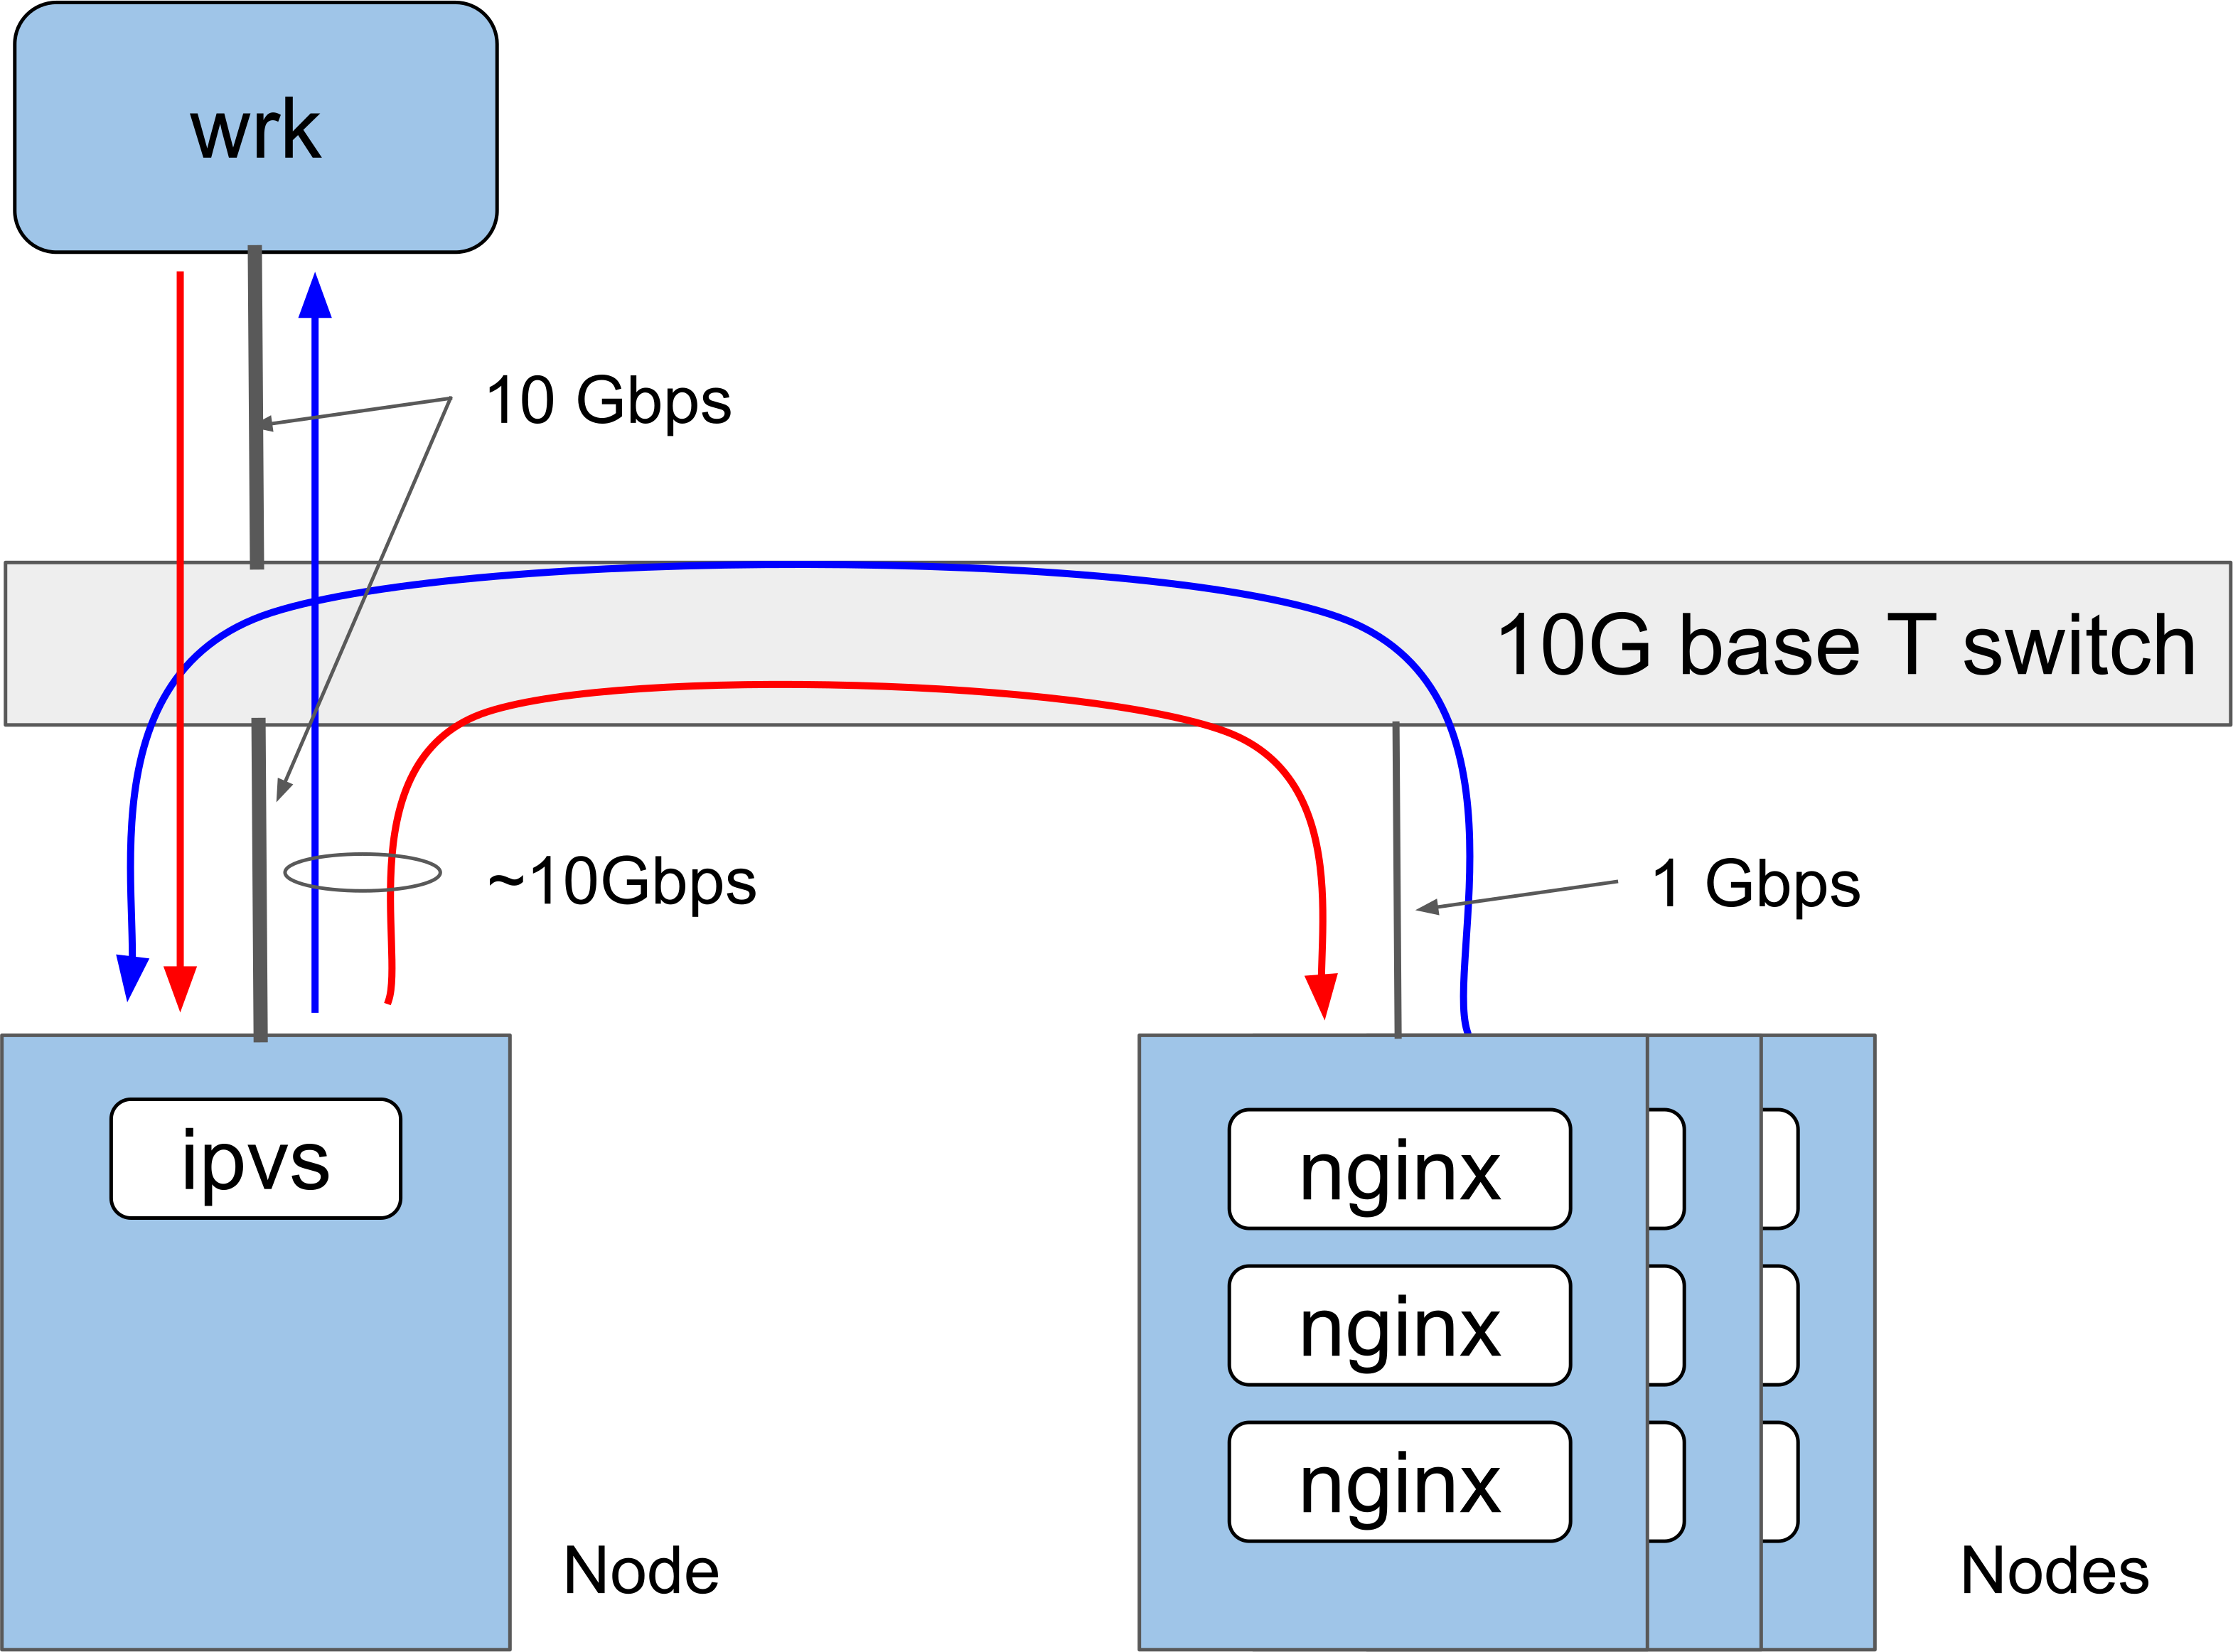
\includegraphics[width=0.8\columnwidth]{Figs/bench_10g}
  \caption{Physical configuration for 10Gbps measurement.}
  \label{fig:bench_10g}
\end{figure}

\begin{figure}[h]
  \centering
  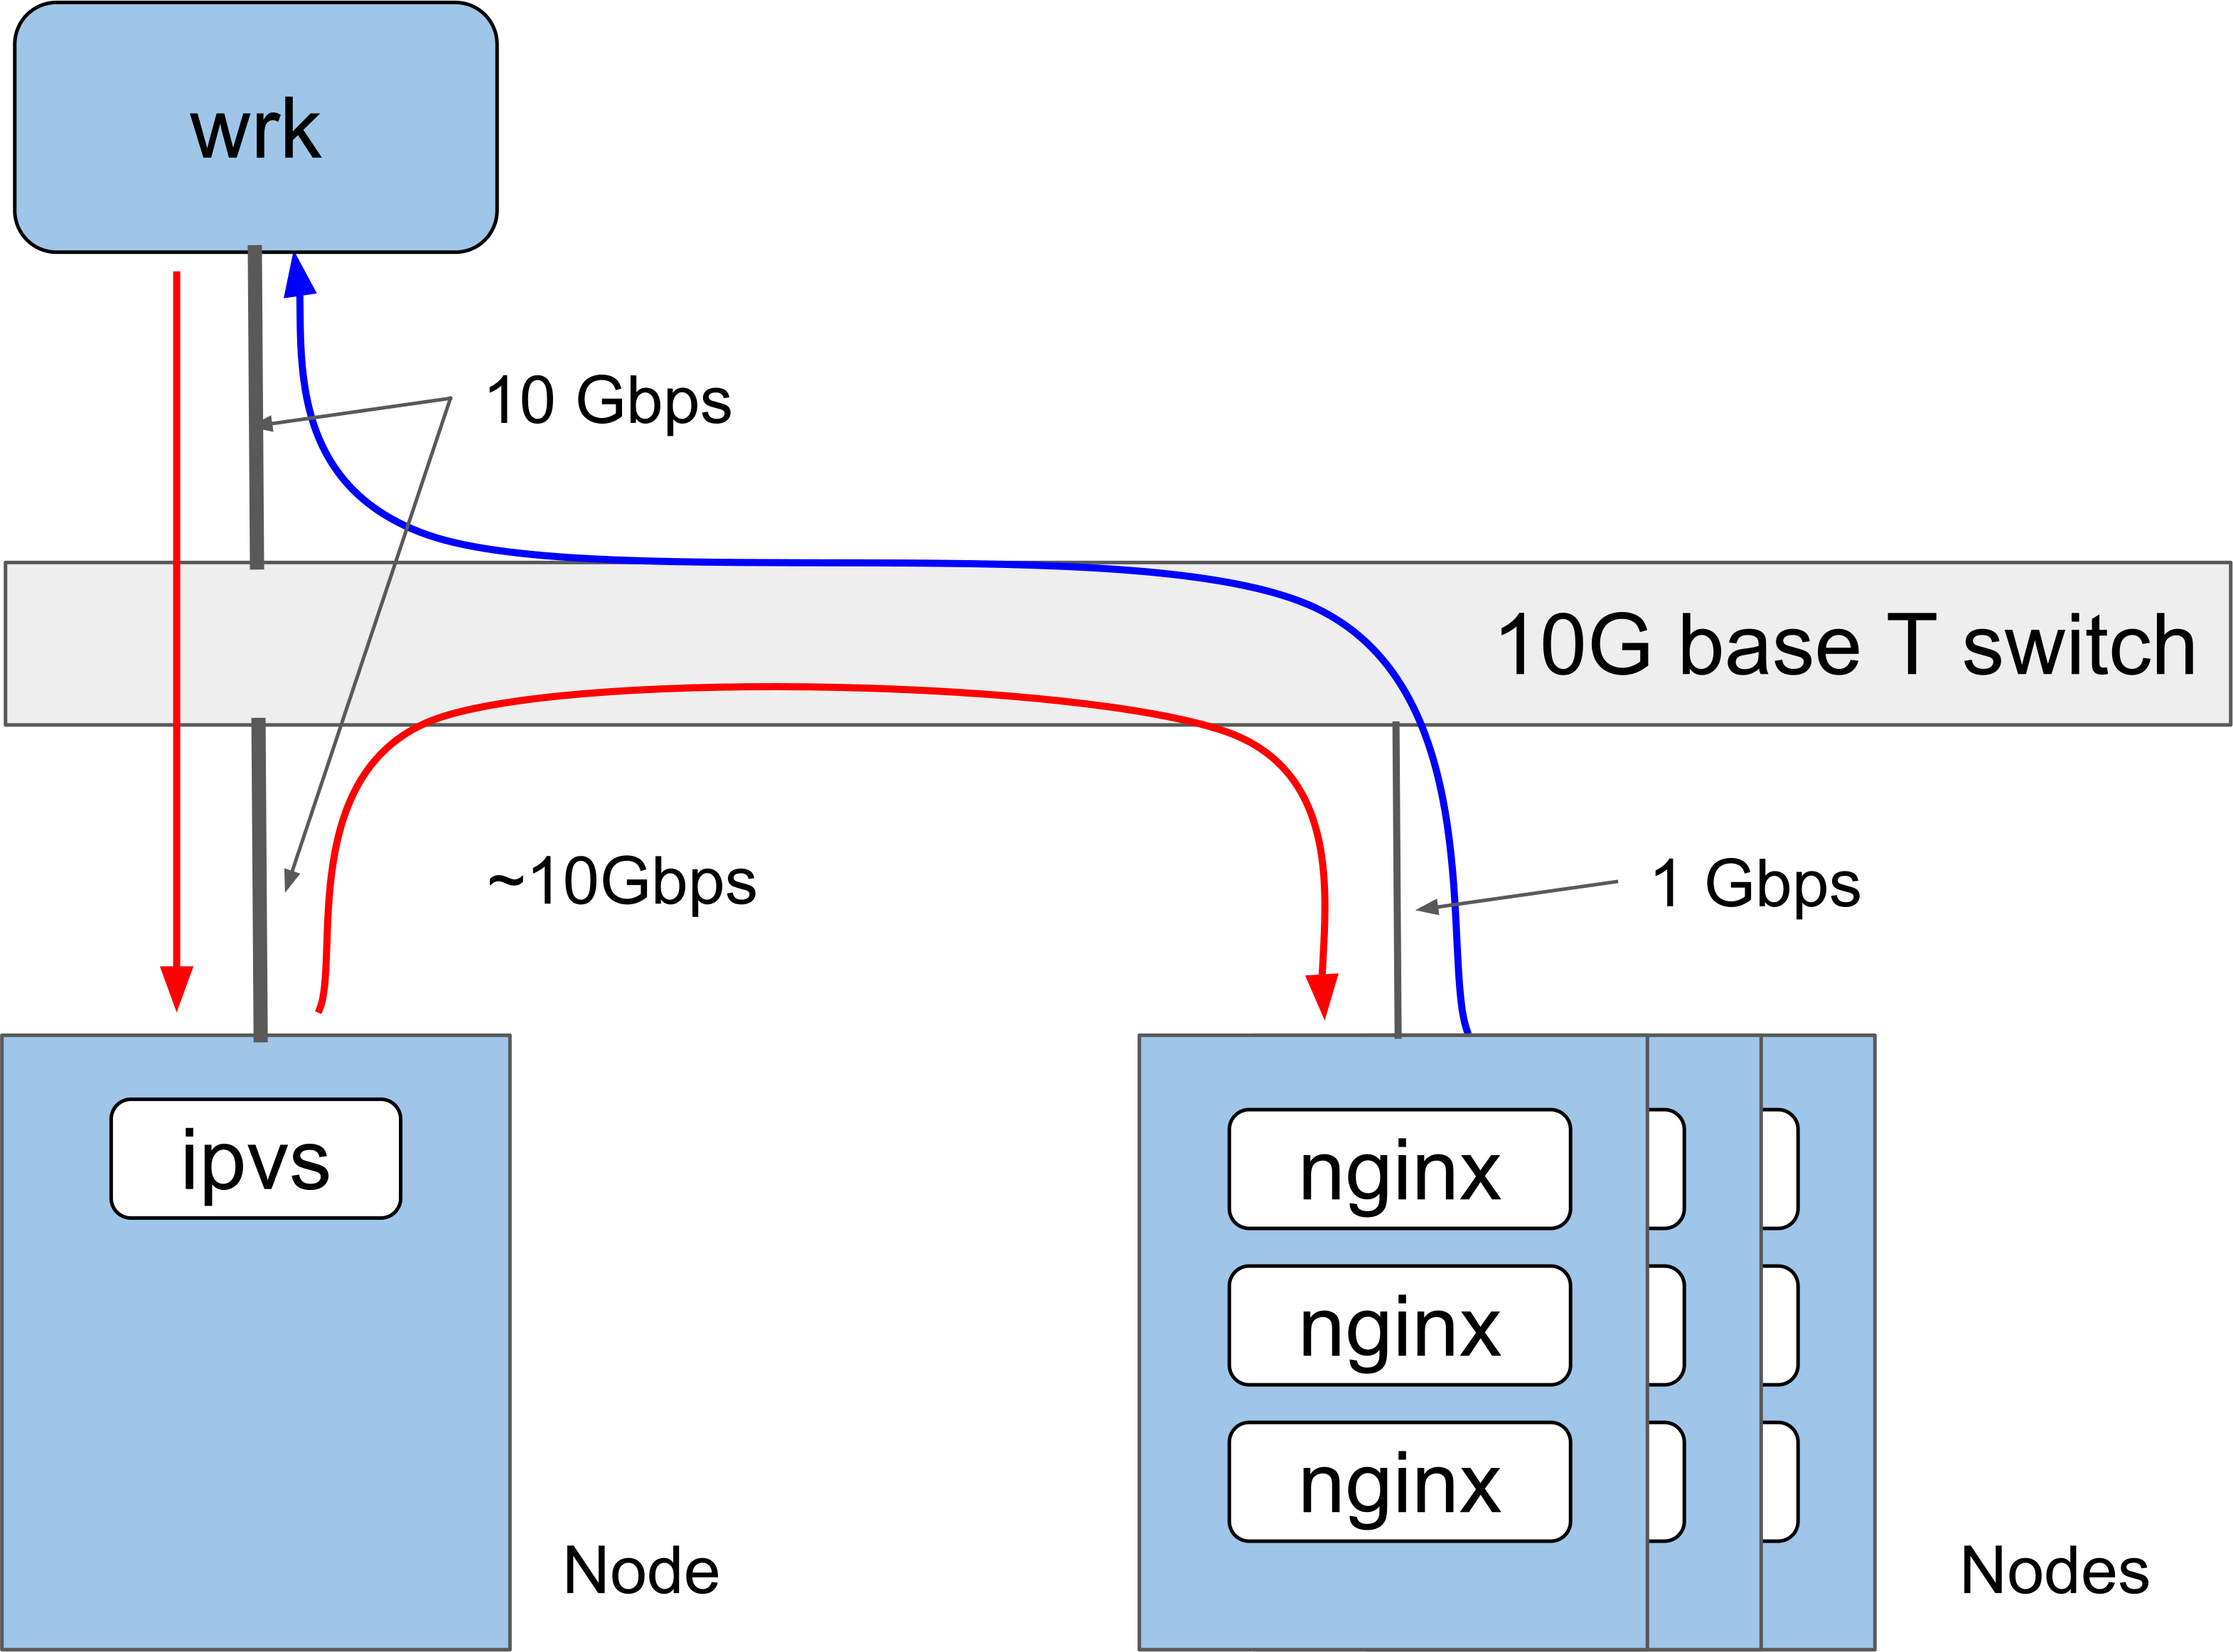
\includegraphics[width=0.8\columnwidth]{Figs/bench_10g_l3dsr}
  \caption{Physical configuration for L3DSR experiment.}
  \label{fig:bench_10g_l3dsr}
\end{figure}

Figure~\ref{fig:ipvs_l3dsr_10g} shows the throughput of ipvs-nat ipvs-tun and iptable DNAT.
While the ipvs-tun showed better performance level than ipvs-nat, the iptables DNAT show yet better peformance level.
The limiting factor for the ipvs-tun and ipvs-nat case seem to be the insufficient CPU perwar for the node.
 


\begin{figure}[h]
  \centering
  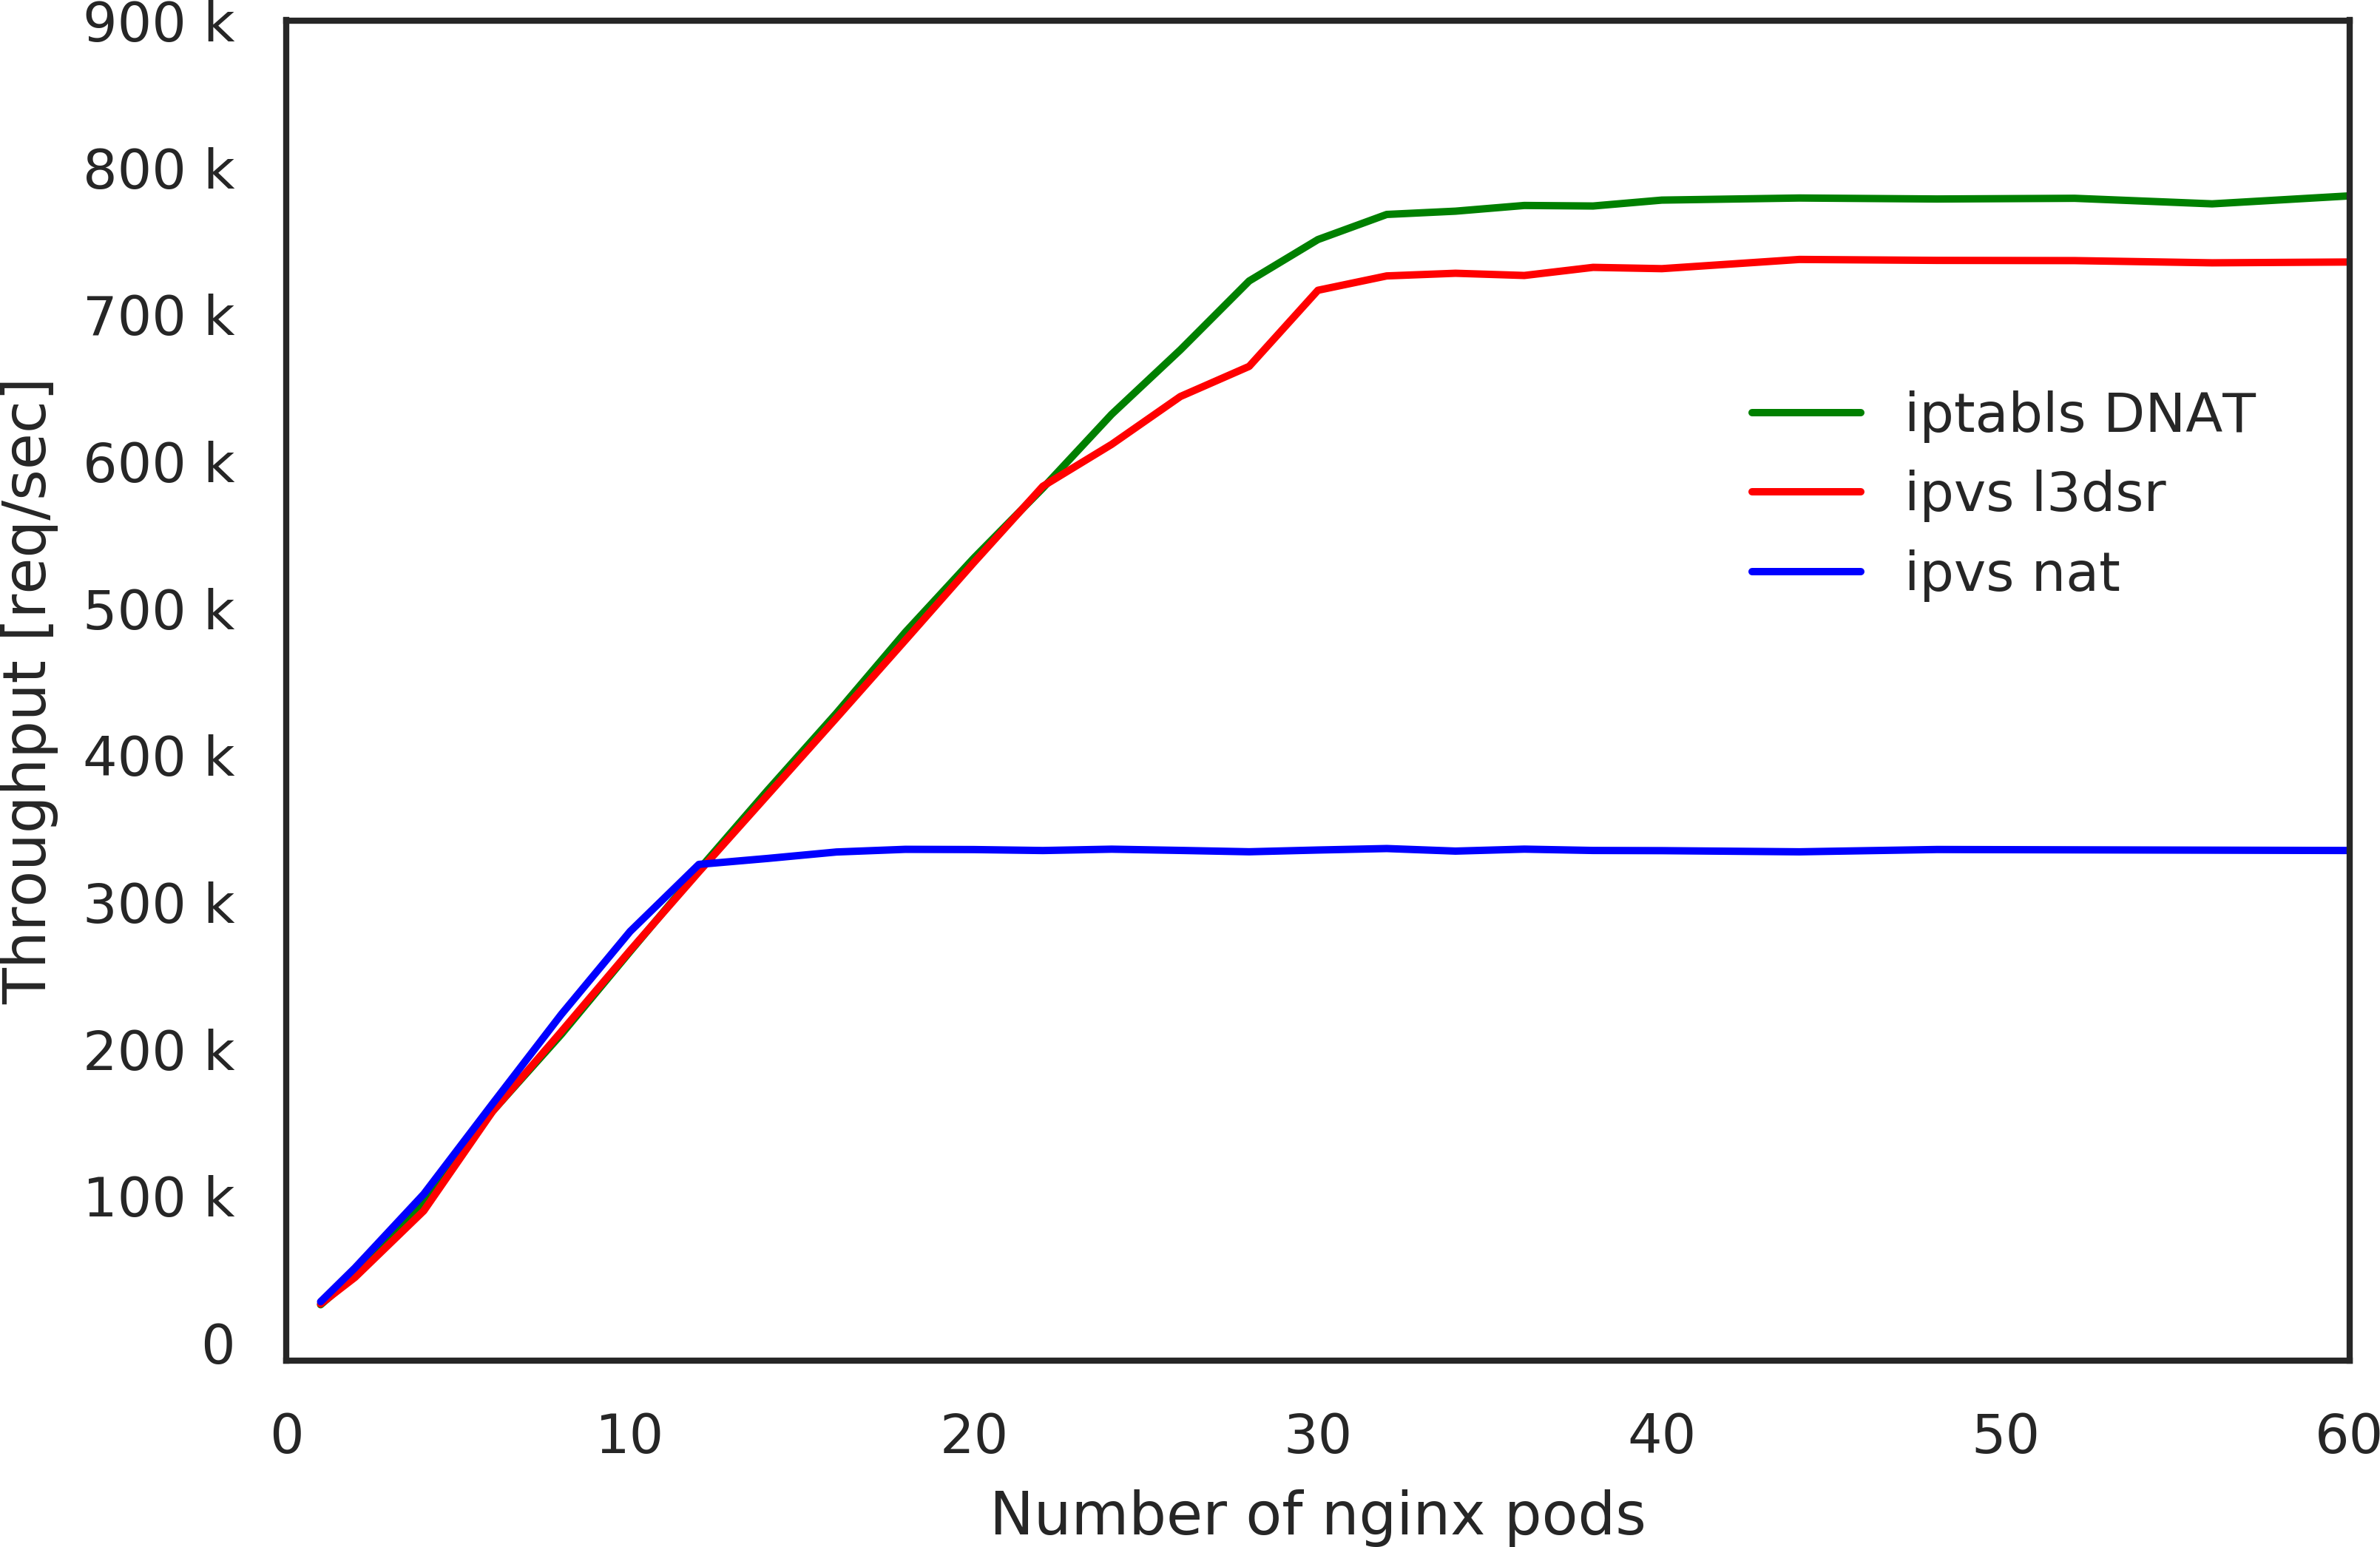
\includegraphics[width=0.8\columnwidth]{Figs/ipvs_l3dsr_10g}
  \caption{Throughput of ipvs l3dsr @10Gbps.}
  \label{fig:ipvs_l3dsr_10g}
\end{figure}

Figure~\ref{fig:ipvs_l3dsr_10g.png} shows the throughput of the ipvs-tun, ipvs masqurade mode togther with iptables DNAT.

\FloatBarrier
\section{Throuput of ipvs-nat, ipvs-tun and iptables DNAT}

\begin{figure}[h]
  \centering
  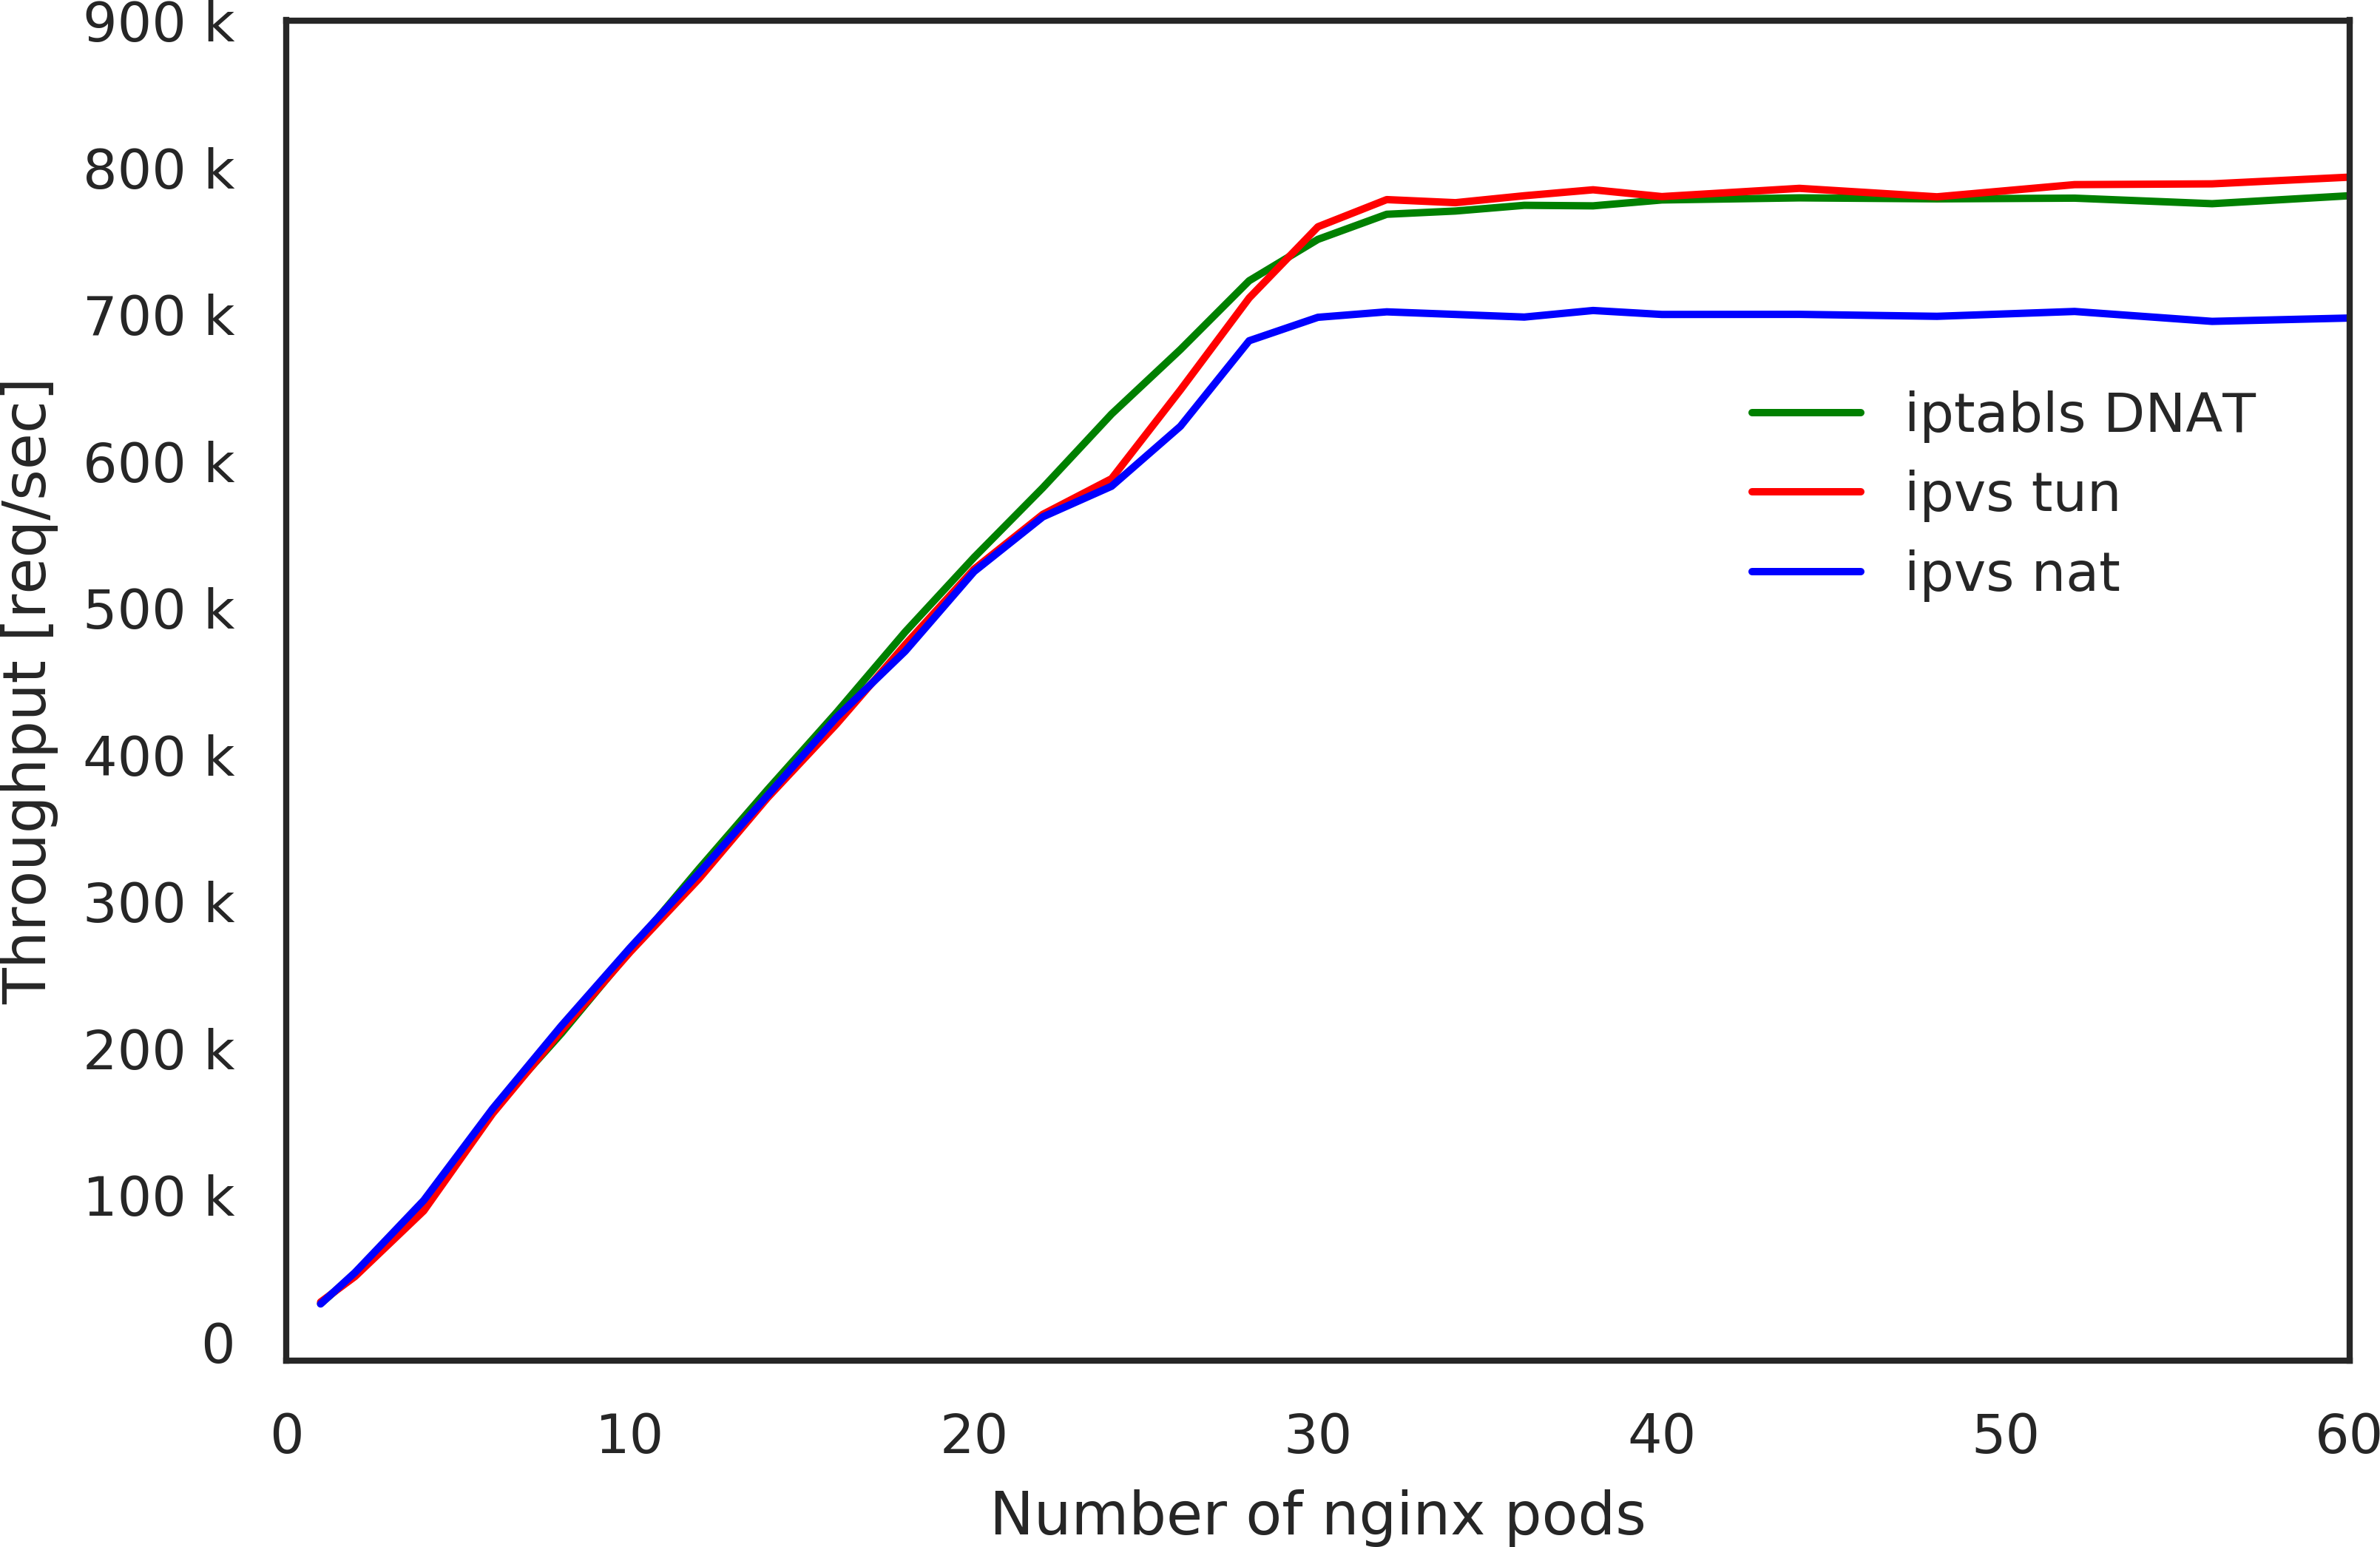
\includegraphics[width=0.8\columnwidth]{Figs/ipvs_node_l3dsr_10g}
  \caption{Throughput of ipvs in node name space.}
  \label{Figs/ipvs_node_l3dsr_10g}
\end{figure}


\FloatBarrier
\section{XDP load balancer}

\section{Summary}



